\documentclass{standalone}
\usepackage{tikz,amsmath}
\tikzset{block/.style = {draw, fill=white, very thick, rectangle, minimum height=1cm, minimum width=2cm},}
\tikzset{sum/.style= {draw, fill=white, very thick, circle, node distance=1cm},}
\begin{document}
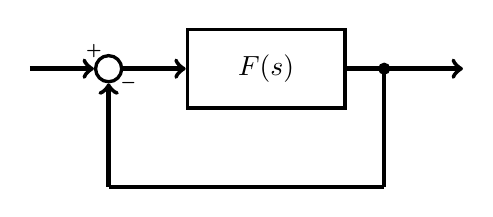
\begin{tikzpicture}[scale=2]
    \node[sum](sum)at(-1,0){};
    \draw[->,ultra thick](-1.5,0)--(sum.180)node[above]{$\scriptscriptstyle\boldsymbol{+}$};

    \node[block, right of=sum, node distance=2cm](g){$F(s)$};

    \draw[->,ultra thick](sum.0)--(g.180);
    \draw[-,ultra thick](g.0)--(0.75,0);
    \filldraw[black](0.75,0)circle(1pt);

    \draw[->,ultra thick](0.75,0)--(1.25,0);
    \draw[-,ultra thick](0.75,-0.75)--(0.75,0);
    \draw[-,ultra thick](0.75,-0.75)--(-1,-0.75);

    \draw[->,ultra thick](-1,-0.75)--(sum.270)node[right]{$\scriptscriptstyle\boldsymbol{-}$};
\end{tikzpicture}
\end{document}